\begin{figure}[H]
\centering
	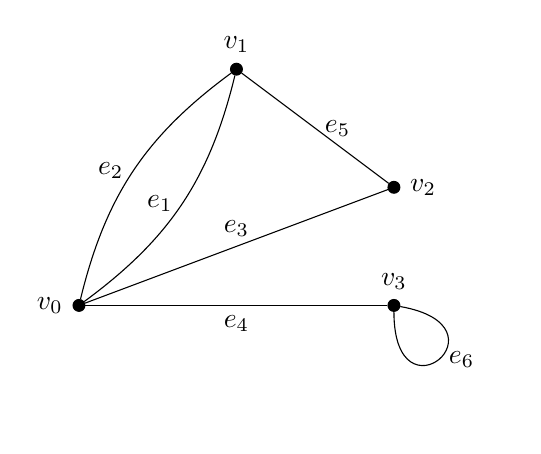
\begin{tikzpicture}[every loop/.style={}]
      \tikzset{enclosed/.style={draw, circle, inner sep=0pt, minimum size=.15cm, fill=black}}
%% Vertices
      	\node[enclosed, label={left: $v_0$}] (v0) at (0,0) {};
      	\node[enclosed, label={above: $v_1$}] (v1) at (2,3) {};
    	\node[enclosed, label={right: $v_2$}] (v2) at (4,1.5) {};
  	    \node[enclosed, label={above: $v_3$}] (v3) at (4,0) {};
%Edges
		\path (v0) edge [bend right=20] node[midway, left] {$e_1$} (v1);
		\path (v1) edge [bend right=20] node[midway, left] {$e_2$} (v0);
		\path (v0) edge node[midway, above] {$e_3$} (v2);
		\path (v0) edge node[midway, below] {$e_4$} (v3);
		\path (v1) edge node[midway, right] {$e_5$} (v2);
		\path (v3) edge [out=270,in=350,looseness=35] node[right] {$e_6$} (v3);
	\end{tikzpicture}
	\caption{En pseudograf med et loop}
	\label{fig.pseudo}
\end{figure}
